% --------------------------------------------------------------
% This is all preamble stuff that you don't have to worry about.
% Head down to where it says "Start here"
% --------------------------------------------------------------
 
\documentclass[12pt,a4paper,twoside]{article}
\usepackage[margin=1in]{geometry} 
\usepackage{amsmath,amsthm,amssymb,listings,graphicx}
\usepackage[usenames,dvipsnames]{xcolor}
\usepackage{fancyhdr}
 
\pagestyle{fancy}
\fancyhf{}

 
\newcommand{\N}{\mathbb{N}}
\newcommand{\Z}{\mathbb{Z}}
\newcommand{\set}[1]{\ensuremath{\left\{{#1}\right\}}}
\newcommand{\bracket}[1]{\ensuremath{\left [{#1}\right]}}
\newcommand{\brocket}[1]{\ensuremath{\left\langle{#1}\right\rangle}}
\newcommand{\norm}[1]{\left\|{#1}\right\|}
\newcommand{\ceil}[1]{\ensuremath{\left\lceil {#1}\right\rceil}}
\newcommand{\floor}[1]{\ensuremath{\left\lfloor {#1}\right\rfloor}}
\newcommand{\paren}[1]{\ensuremath{\left({#1}\right)}}
 
\newenvironment{exercise}[2][Exercise]{\begin{trivlist}
\item[\hskip \labelsep {\bfseries #1}\hskip \labelsep {\bfseries #2.}]}{\end{trivlist}}
\newcommand{\solution}{\medskip\noindent{\textit{Solution:}}\quad}

\definecolor{dkgreen}{rgb}{0,0.6,0}
\definecolor{gray}{rgb}{0.5,0.5,0.5}
\definecolor{mauve}{rgb}{0.58,0,0.82}

\lstset{frame=tb,
  language=R,
  aboveskip=3mm,
  belowskip=3mm,
  showstringspaces=false,
  columns=flexible,
  basicstyle={\small\ttfamily},
  numbers=none,
  numberstyle=\tiny\color{gray},
  keywordstyle=\color{blue},
  commentstyle=\color{dkgreen},
  stringstyle=\color{mauve},
  breaklines=true,
  breakatwhitespace=true,
  tabsize=3
} 

\lhead{\color{Maroon}David Plotz working with Taha}
\rhead{\color{Maroon}Stat. 6509}
\chead{\color{Maroon}Final Project}
\cfoot{\thepage}

\begin{document}

% --------------------------------------------------------------
%                         Start here
% --------------------------------------------------------------
\section{Introduction}
In this report we will create a regression model to predict the wages of a worker in the United States given several predictor variables. We first aggregated and created new predictor variables. We then selected a model that seemed to give a good fit to the log wages. Using this model, we were able to predict the wages of an individual to an accuracy of plus or minus three dollars 90\% of the time. Afterwards, I used cross-validation to see how much of our model could be constructed using only a partial sample of the data. Using the model created from the cross-validation procedure produced slightly better predictions to an accuracy of plus or minus two dollars and eighty cents 90\% of the time. 

The predictor variables included many indicator variables. We decided to group these indicator variables into three different groups. The first group, which we called region, contained the three indicator variables: west, northcen, and south. The second group, which we called business type, contained the indicator variables for contruction, non-durable manufacturing, transportation/communication/utility, wholesale/retail, services and professional services. The final group, which we called job type, included the indicators professional, clerical, and service. We also included the interaction between several of these predictor variables to see if any of these interactions are also useful for prediction, including the interaction of education with itself (i.e., the square of eduction), the interaction of education with experience, and the interaction between how long someone has been at a company and whether they live in a metropolitan area. We were also interested in the way gender could be used as an interaction and we thewrefore included several interactions with gender including the interaction with race, marital status, business type, and job type.
\section{Cleaning the Data}	
Before starting to make our model, we first checked for outliers in our data set. One of the data points was particularly troubling as the person was making less than the minimum wage. We decided at the outset to drop this data point from our data set because we figured it was probably an error in the data collection methods and could only disrupt our analysis.
	
After deleting this outlier, we examined the histogram of wages. As you can see, below to the left, the wages are skewed to the right, we therefore used the log of wages instead, which I have plotted on the left.
\begin{center}
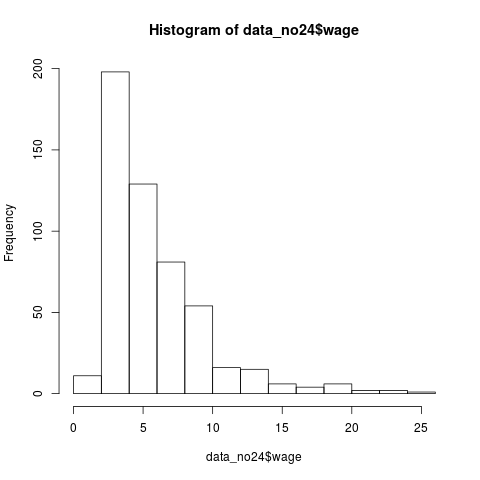
\includegraphics[scale=.4]{plot2.png}
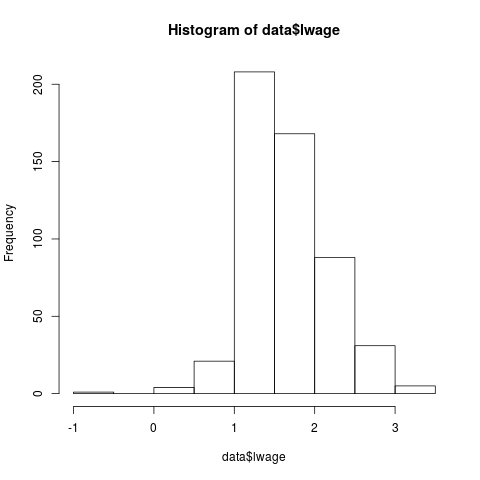
\includegraphics[scale=.4]{plot1.png}
\end{center}

Before including the interactions into the model, we wanted to make sure that a linear interaction was appropriate for each of the numeric explanatory variables. What we found was that experience, education and tenure all showed curvature. We therefore included education squared, experience squared, and the log transformation of tenure into our model. Below I have plotted tenure versus log of wages and log of tenure versus log of wages\\
\begin{center}
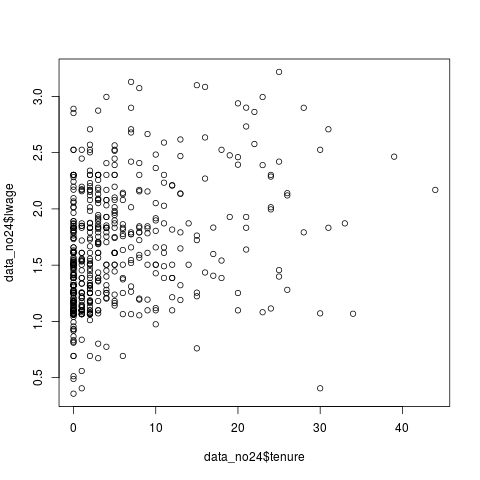
\includegraphics[scale=.4]{tenure.png}
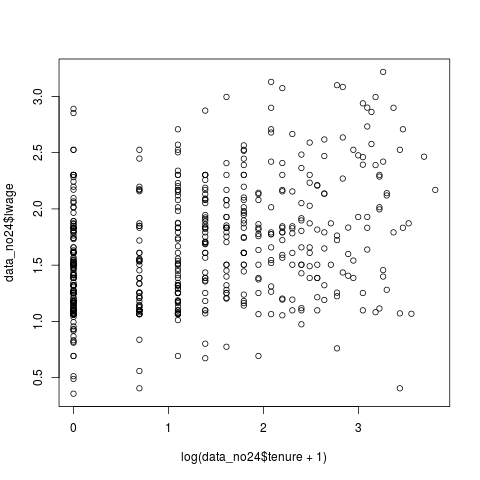
\includegraphics[scale=.4]{logtenure.png}
\end{center}

As one would imagine, there was a strong correlation between tenure and experience, as the plot below shows. However the correlation between them was less than 50 percent, and we therefore decided that both experience and tenure can be included in our model.\\
%\includegraphics[scale=.9]{Rplot02}
\begin{center}
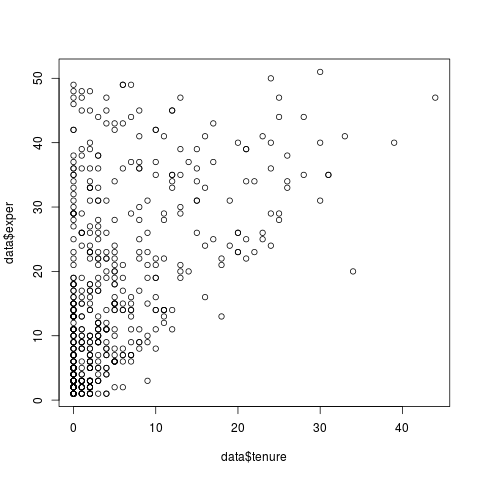
\includegraphics[scale=.3]{cor.png}
\end{center}

Finally, we were ready to include the interactions in our model. The full model included over 20 different predictor variables. After running the linear regression algorithm on the full data set. We found that the adjusted R-squared was 0.5577.

At this point, we wanted to check for normality and homoscedasticity. Looking at the normal plot below, it is easy to see that our residuals are quite normal. Using the Shapiro-Wilk test indicated that W was 0.9875, and because our data set is quite large, we conclude that the data is approximately normally distributed even though the p-value was small. Using the Breusch-Pagan test we checked for homoscedasticity, but unfortunately, there appeared to be variation in the variance. However, since we have already taken the log of the wages, we feel that there is not much more we can do.\\
\begin{center}
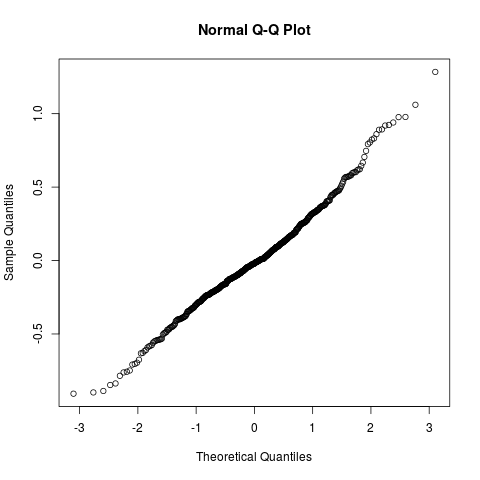
\includegraphics[scale=.4]{norm.png}
\end{center}

\section{Choosing a Model}

After examining the full model, we used the adjusted R-squared to take out predictor variables, I was able to remove nine predictor variables and improve my adjusted R-squared score to 0.5606.\\

We also used step AIC to remove predictor variables. The step AIC procedure gave a similar result as the adjusted R-squared procedure but removed three of the interactions. This caused the adjusted R-squred score decrease to 0.559. However, it was our view that because there was significantly fewer predictor variables, the model chosen by step AIC would provide a better fit. Our final model included the following predictor variables:\\ 

\begin{verbatim}
educ                                              0.223008    
educsq                                            0.002303 ** 
exper                                             1.01e-07 ***
expersq                                           8.88e-08 ***
log.tenure                                        0.204467    
as.factor(numdep)1                                0.021732 *  
as.factor(numdep)2                                0.123353    
as.factor(numdep)3                                0.523771    
as.factor(numdep)4                                0.006330 ** 
as.factor(numdep)5                                0.085341 .  
as.factor(numdep)6                                0.500900    
as.factor(metro)suburb                            2.36e-05 ***
as.factor(marital.st)single                       0.232568    
as.factor(gender)male                             0.000356 ***
as.factor(business.type)ndurman                   0.566093    
as.factor(business.type)other                     0.520166    
as.factor(business.type)profserv                  0.590710    
as.factor(business.type)services                  0.017377 *  
as.factor(business.type)trade                     0.001464 ** 
as.factor(business.type)trcommpu                  0.458339    
as.factor(job.type)other                          0.447437    
as.factor(job.type)profocc                        0.007384 ** 
as.factor(job.type)servocc                        0.021391 *  
as.factor(marital.st)single:as.factor(gender)male 0.001311 ** 
log.tenure:as.factor(gender)male                  0.003774 ** 
\end{verbatim}

\section{Making Predictions} 
After selecting the model, we were ready to test it using a hold-out sample. I removed 100 samples from the original data set. I then ran the regression using the remaining samples. I then used the returned model to make predictions on the hold-out sample. What I found is that slightly more than 90\% of the samples were within the 95\% confidence limits. And in fact, over 90\% of the actual log wages were within 0.5 of the predicted log wages. However, using the log wages makes it difficult to interpret, so what I did was transformed the log wages back to the normal wages to see how well our model performed. Below, you can see a sample of how the predictions for actual wages fared:

\begin{verbatim}

     real      pred         diff
441 11.25 11.411433  0.161432723
173  5.25  5.794939  0.544939457
399 10.92  6.594707  4.325293232
339 12.22  9.022146  3.197854444
132  5.00  6.389291  1.389290920
470  3.00  3.862416  0.862416016
110  9.80  6.883612  2.916388016
209  6.15  4.451548  1.698452287
250  3.00  2.539863  0.460136961
452  3.25  2.695256  0.554743794
387  4.14  3.935313  0.204687239
440 20.00  5.365481 14.634518659
480  3.25  3.692755  0.442755145
428  2.88  2.612865  0.267135109
469  8.00  5.381957  2.618043097
474  3.00  2.792172  0.207828145
\end{verbatim}

What I found from this analysis was that with 90\% confidence, I could perdict the wages of a person to within a range of plus or minus three dollars. This seemed to me like a fairly poor performance and may be due to the lack of homoscedasticity. 

\section{Using Cross-Validation to Model Select} 
Before making a final analysis of the data, I was interested to see how much of our model was based simply on random noise in the data. What I decided to do was to take the hold-out sample technique one step further, and do a full-blown cross-validation of the model. I therefore split my data as before, using a random sample of 100 data points to hold-out as a test set, and used the remaining samples to make my model.

I ran and recorded the results of doing the cross-validation ten times. Here is a sample of the outcomes:

\begin{verbatim}
                                          Df Sum of Sq    RSS     AIC
- as.factor(numdep)                        6    1.3869 54.068 -994.21
- log.tenure:as.factor(metro)              1    0.6061 53.287 -991.12
- as.factor(marital.st):as.factor(gender)  1    1.7596 54.440 -980.95
- exper                                    1    2.5766 55.257 -973.88
- expersq                                  1    2.5978 55.278 -973.69
- as.factor(job.type)                      3    3.5408 56.221 -969.66
- as.factor(business.type)                 6    5.7450 58.426 -957.39
- educsqr                                  1    4.9644 57.645 -953.78
\end{verbatim}

\begin{verbatim}
                                          Df Sum of Sq    RSS     AIC
- as.factor(race):as.factor(gender)        1    0.3238 56.671 -969.87
- log.tenure:as.factor(metro)              1    0.4261 56.774 -969.02
- as.factor(marital.st):as.factor(gender)  1    1.4343 57.782 -960.65
- expersq                                  1    3.0707 59.418 -947.39
- exper                                    1    3.1400 59.487 -946.84
- as.factor(job.type)                      3    3.7829 60.130 -945.73
- as.factor(business.type)                 6    4.5862 60.934 -945.43
- educsqr                                  1    5.7390 62.086 -926.52
\end{verbatim}

\begin{verbatim}
                                          Df Sum of Sq    RSS     AIC
- educ:exper                               1    0.2383 56.224 -973.64
- log.tenure:as.factor(metro)              1    0.4025 56.388 -972.25
- educsqr                                  1    0.9689 56.954 -967.51
- as.factor(marital.st):as.factor(gender)  1    1.7491 57.734 -961.04
- expersq                                  1    1.8018 57.787 -960.61
- as.factor(job.type)                      3    3.3688 59.354 -951.90
- as.factor(business.type)                 6    4.7665 60.752 -946.85
\end{verbatim} 

What I found from doing this analysis was that, indeed, the sample that was used to create the model had a huge impact upon the final variables chosen. However, there was still some consistency in the final variables chosen. What I decided to do was create a model that was as consistent across the various cross-over results and see what this model implied. The final model, that I chose from using this method is posted below (where education was added for reasons of interpretability):

\begin{verbatim}
educ                                              0.346500    
educsqr                                           0.004401 ** 
exper                                             7.07e-07 ***
expersq                                           6.80e-07 ***
log.tenure                                        1.38e-07 ***
as.factor(metro)suburb                            0.170557    
as.factor(marital.st)single                       0.109558    
as.factor(gender)male                             1.20e-14 ***
as.factor(business.type)ndurman                   0.401462    
as.factor(business.type)other                     0.569284    
as.factor(business.type)profserv                  0.483175    
as.factor(business.type)services                  0.016994 *  
as.factor(business.type)trade                     0.001492 ** 
as.factor(business.type)trcommpu                  0.459525    
as.factor(job.type)other                          0.339663    
as.factor(job.type)profocc                        0.006531 ** 
as.factor(job.type)servocc                        0.013561 *  
log.tenure:as.factor(metro)suburb                 0.052529 .  
as.factor(marital.st)single:as.factor(gender)male 0.000206 ***
\end{verbatim}

The predictor variables that were not included in this model often showed up in a particular representation. For example, the race predictor variable showed up in about half of the models. However, the variables included here, with the exception of the linear education, were in all of the models chosen by the step AIC procedure.

Using this model, I again tried to make predictions on the remaining 100 samples taken out as a test-set. Here we were actually able to see a slight improvement from our bigger model using the full data set. Instead of being able to predict with 90\% confidence the wage within a range of plus or minus three dollars, we were able to make a 90\% confident prediction at plus or minus two dollars and eighty cents. However, this still seems like the accuracy is not high enough to be useful for many tasks.
\section{Final Analysis}
As I have shown, the random subset of data chosen to make a model has a huge impact on the final model chosen. Models with more predictor variables seemed to overfit the data. While models with more predictor variables generally had a lower MSE score, when they were used to make predictions on data not seen before they performed slightly worse than simpler models. 

With this said, there was still a fair amount of constitency across the various models. In my analysis, the only two predictor variables that were not included were race and the number of dependents. Apparently, neither of these make a significant impact upon a persons wages, all else held equal. Of the dozen or so interactions that we examined, only two were consistently in all the models: the interaction between tenure and whether someone lived in a metropolitan area or not, and the interaction between gender and marital status. Apparently, if you work at a job for a long time outside of metropolitan area, you will make less than someone who works in a metropolitan area. Also, according to my analysis, single males made less than married men. Finally, the most important predictors were still the ones that ones that we would normally associate with high wages: education, experience, tenure, and being a male.   





\end{document}
